\documentclass[../delivery_hospital_report.tex]{subfiles}
\graphicspath{ {images/}{../images/}{../../images/} }

\begin{document}

A Escola Politécnica e Hospital Universitário da USP vem colaborando para o desenvolvimento de soluções para a área da
saúde. Um dos projetos em desenvolvimento é o Robô Hospitalar [1] que já foi documentado detalhadamente pelo Aluno Vanderson Santos. A equipe da Poli
e do HU vêm realizando reuniões quinzenais para identificação de problemas e
necessidades do hospital, tendo em vista a discussão e a criação conjunta de soluções
customizadas para a realidade Brasileira. Atualmente, a maioria dos equipamentos hospitalares são
importados e os custos elevados [2]. Além disso, o Brasil precisa buscar soluções
adaptadas às suas características específicas do Sistema Único de Saúde (SUS) [3].
Diante deste cenário, a fim de atender às necessidades atuais do HU, este projeto tem
como proposta o desenvolvimento de tecnologias para a fabricação de dois tipos de
equipamentos: Dispensador Automático de Medicamentos e Bicicleta
Cicloergométrica. Embora aplicação e funcionalidades distintas, ambos equipamentos
possuem elementos em comum, incluindo estrutura mecânica, módulos elétricos e
eletrônica embarcada. A ideia é a constituição de uma equipe multidisciplinar de
alunos das áreas de engenharia elétrica, mecatrônica e de mecânica para realizar o
estudo de tecnologias e materiais adequados para a fabricação de equipamentos
hospitalares. Um fator essencial é a interação com os médicos e especialistas em
saúde, em especial dos setores de farmácia e de fisioterapia. Pois, um dos principais
desafios para o desenvolvimento tecnológico na área de saúde é a correta
compreensão do ambiente hospitalar, as necessidades operacionais e os problemas
específico da realidade dos hospitais do país, incluindo escassez de recursos e
capacitação técnica dos profissionais de saúde.
Um dos maiores problemas nos grandes hospitais da atualidade é a sobrecarga de trabalhos desnecessários, até mesmo fútil, como transporte de medicamentos e exames, para profissionais altamente qualificados. Nos últimos tempos, principalmente por conta do início da Pandemia do COVID19, o número de pessoas que vem frequentando os hospitais é cada vez maior. Em momentos como esses, profissionais da área da saúde perder tempo com serviços automatizáveis corroboram para a ineficiência e demora no atendimento em ambientes hospitalares, que em geral pode custar vidas.

Para contornar esses problemas de automação hospitalar, é cada vez mais comum a utilização de robôs hospitalares, que cumprem a função de realizar trabalhos repetitivos e banais. Isso garante que profissionais da saúde utilizem mais do seu tempo de trabalho exercendo os seus deveres profissionais que fazem sentido com sua profissão. 

Robôs Hospitalares, principalmente graças aos avanços da indústria 4.0, que cumpre funções de automação hospitalar estão cada vez mais em evidência no mercado mundial. Um exemplo disso é robô hospitalar Hospi, que pode ser vista na figura ~\ref{fig: Robô Hospi}, que foi projetado para fazer o transporte de medicamentos por todo um hospital. 


\begin{figure}[h]
\centering
    \caption{Robô Hospi}
    \centering % para centralizarmos a figura
    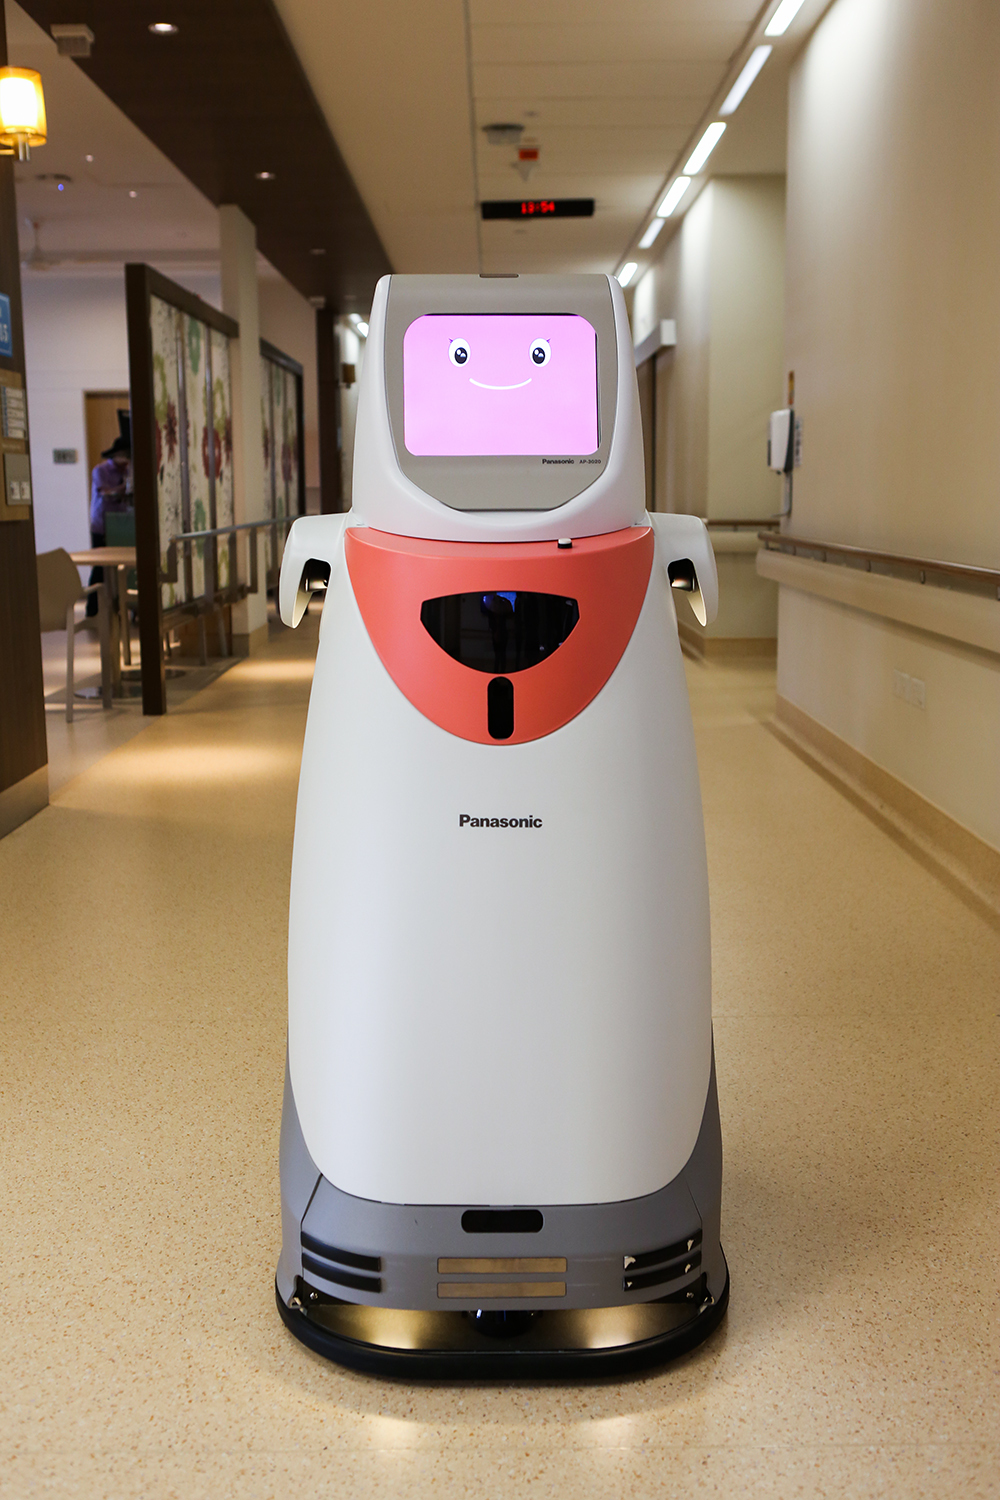
\includegraphics[width=11cm]{hospi.jpg}
    \caption*{Fonte: Business Wire}
    \label{fig: Robô Hospi}
\end{figure}

\end{document}